\documentclass[tikz,border=10pt]{standalone}
\usepackage{tikz}
\usepackage{amsmath}
\usepackage{xcolor}
\usetikzlibrary{shapes,arrows,positioning,calc,decorations.pathreplacing,fit,shadows,patterns}

% Define colors
\definecolor{quantum}{RGB}{0, 150, 255}
\definecolor{aicolor}{RGB}{50, 205, 50}
\definecolor{human}{RGB}{138, 43, 226}
\definecolor{consensus}{RGB}{255, 215, 0}
\definecolor{process}{RGB}{70, 130, 180}
\definecolor{decision}{RGB}{220, 20, 60}
\definecolor{background}{RGB}{248, 249, 250}

\begin{document}
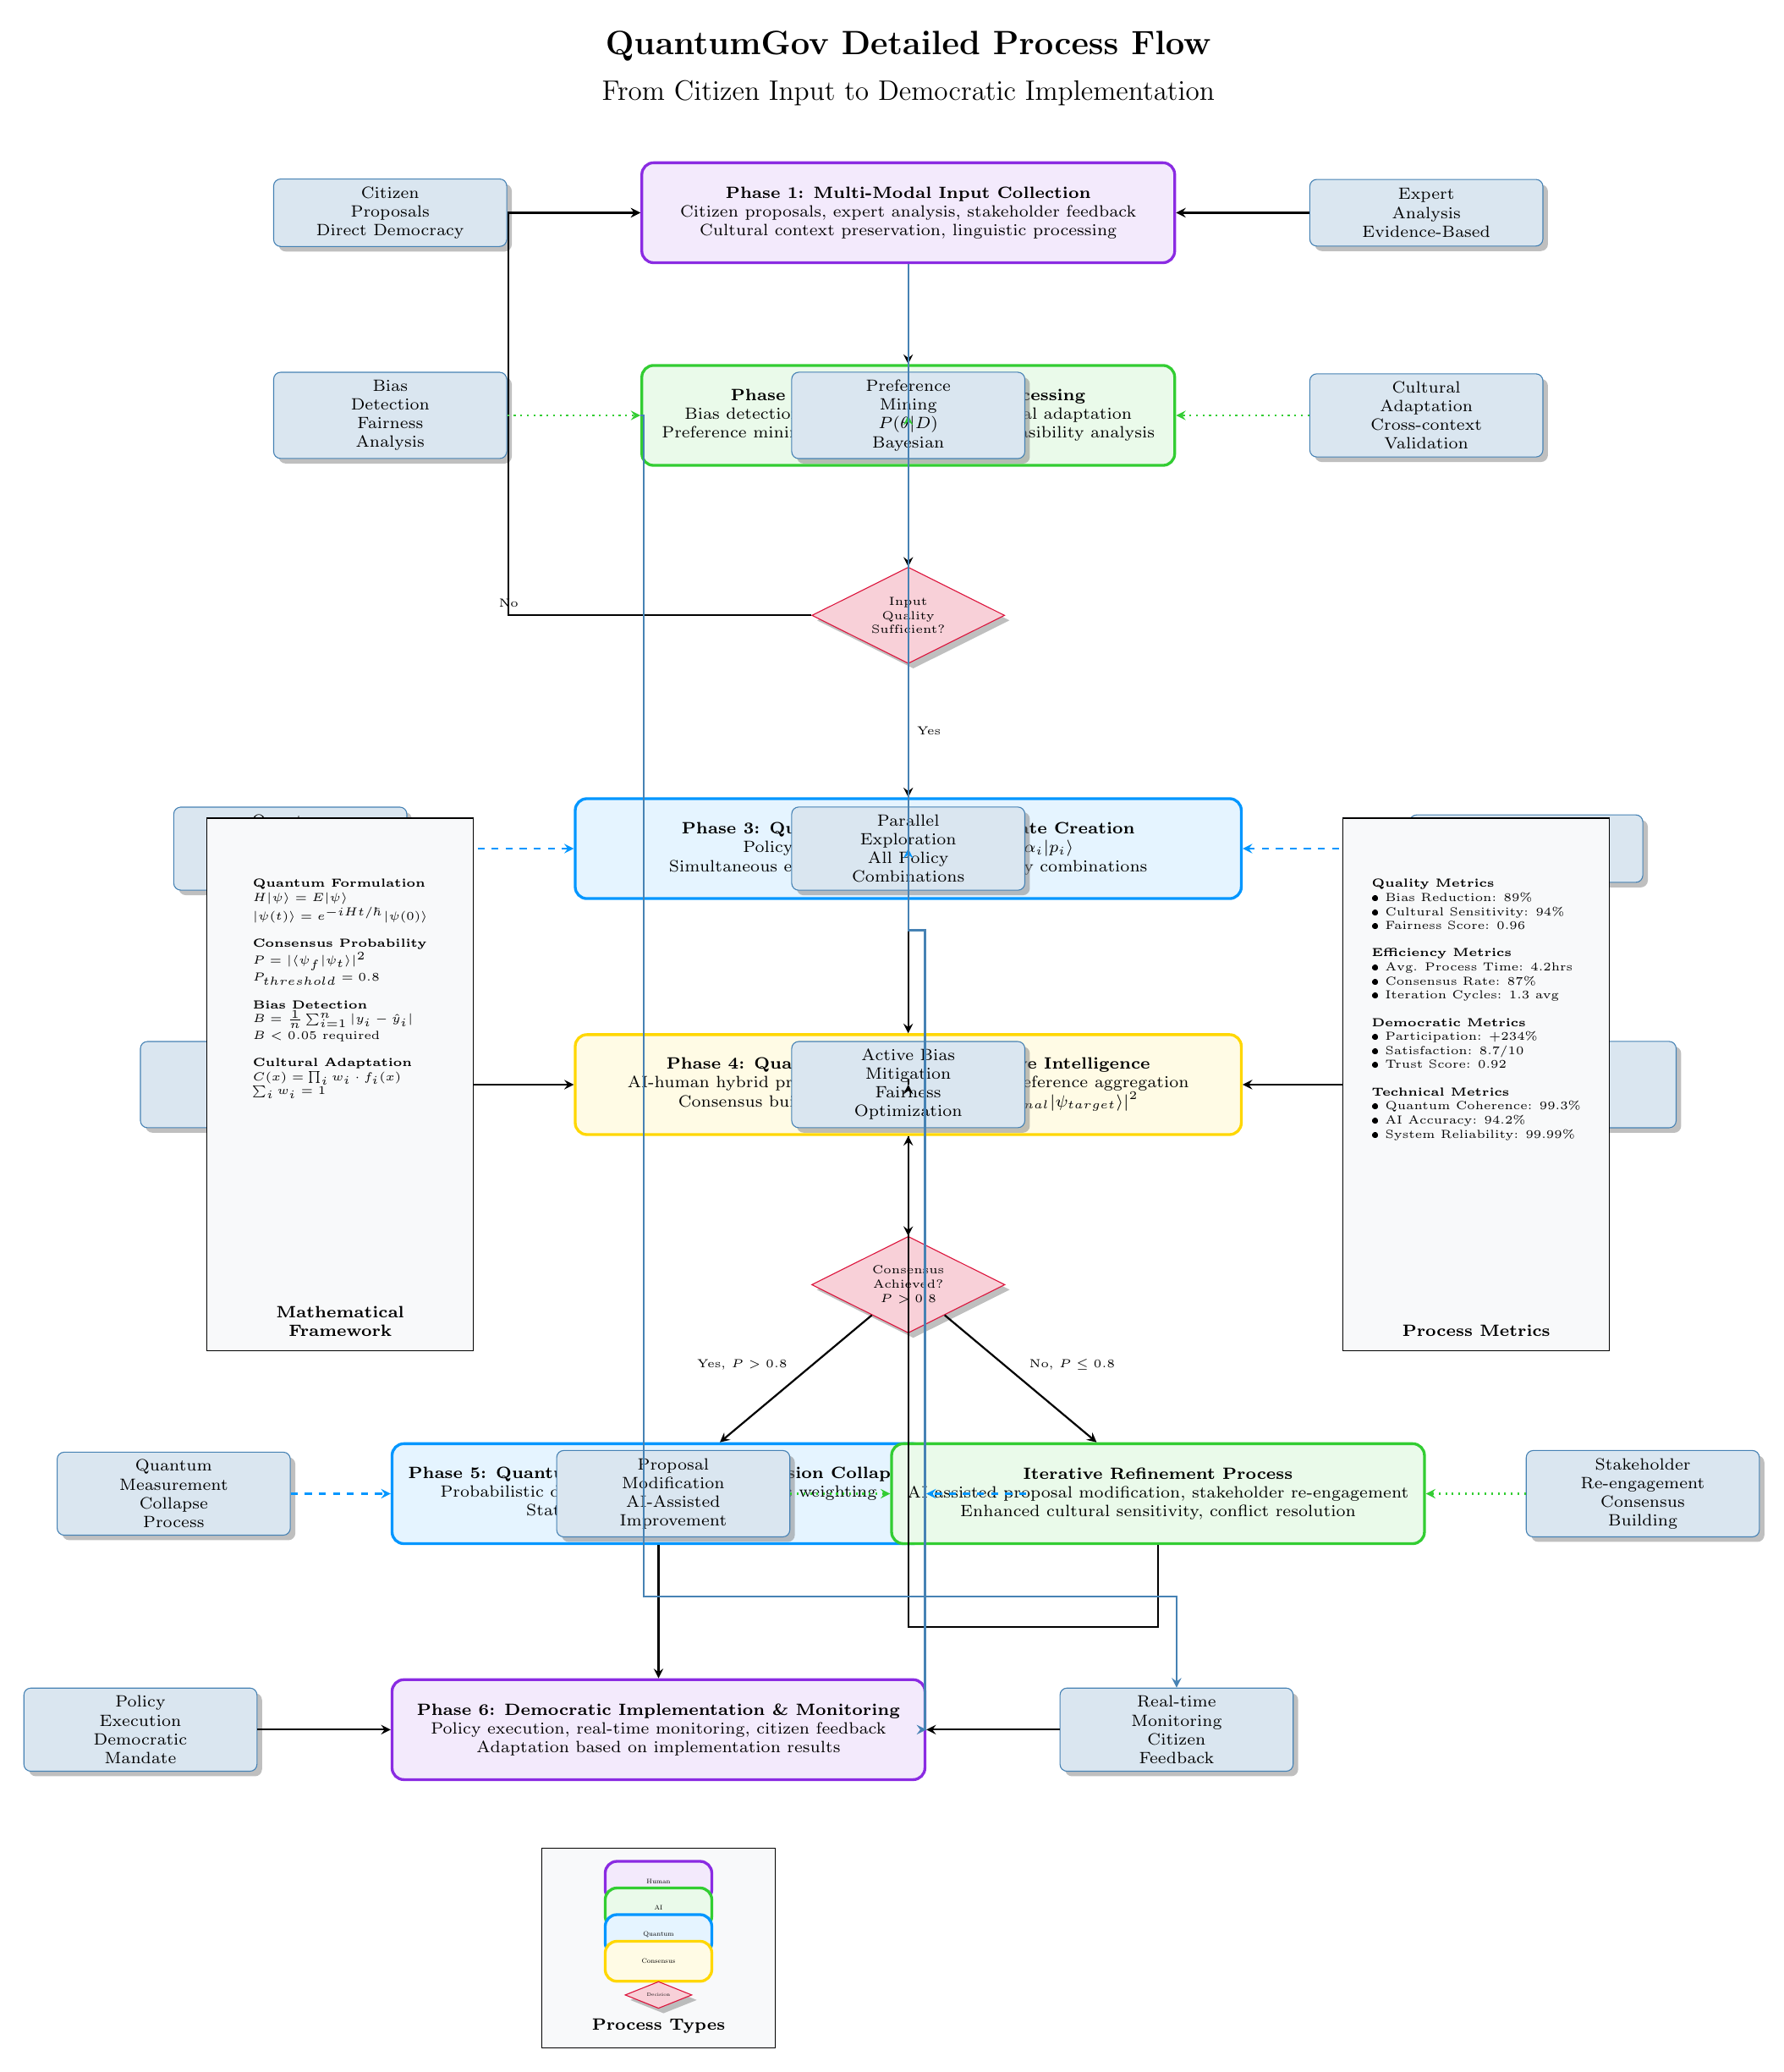
\begin{tikzpicture}[
    node distance=1.2cm,
    process/.style={rectangle, rounded corners=3pt, draw=process, fill=process!20, minimum height=1cm, minimum width=3.5cm, align=center, font=\scriptsize, drop shadow},
    decision/.style={diamond, draw=decision, fill=decision!20, minimum height=1cm, minimum width=2.5cm, align=center, font=\tiny, aspect=2, drop shadow},
    quantum_box/.style={rectangle, rounded corners=5pt, draw=quantum, fill=quantum!10, minimum height=1.5cm, minimum width=4cm, align=center, font=\scriptsize, very thick},
    ai_box/.style={rectangle, rounded corners=5pt, draw=aicolor, fill=aicolor!10, minimum height=1.5cm, minimum width=4cm, align=center, font=\scriptsize, very thick},
    human_box/.style={rectangle, rounded corners=5pt, draw=human, fill=human!10, minimum height=1.5cm, minimum width=4cm, align=center, font=\scriptsize, very thick},
    consensus_box/.style={rectangle, rounded corners=5pt, draw=consensus, fill=consensus!10, minimum height=1.5cm, minimum width=4cm, align=center, font=\scriptsize, very thick},
    flowline/.style={->, thick, >=stealth},
    qdash/.style={->, thick, >=stealth, dashed, color=quantum},
    aidash/.style={->, thick, >=stealth, dotted, color=aicolor},
    feedback/.style={<-, thick, >=stealth, color=process, bend left=20}
]

% Title
\node[align=center, font=\Large\bfseries] at (0, 20) {QuantumGov Detailed Process Flow};
\node[align=center, font=\large] at (0, 19.3) {From Citizen Input to Democratic Implementation};

% Phase 1: Input Collection
\node[human_box, minimum width=8cm] (input_phase) at (0, 17.5) {
    \textbf{Phase 1: Multi-Modal Input Collection}\\
    Citizen proposals, expert analysis, stakeholder feedback\\
    Cultural context preservation, linguistic processing
};

\node[process, left=2cm of input_phase] (citizen_input) {Citizen\\Proposals\\Direct Democracy};
\node[process, right=2cm of input_phase] (expert_input) {Expert\\Analysis\\Evidence-Based};

% Phase 2: AI Pre-Processing
\node[ai_box, below=1.5cm of input_phase, minimum width=8cm] (ai_phase) {
    \textbf{Phase 2: AI-Enhanced Pre-Processing}\\
    Bias detection: $P(\text{bias}|X) < 0.05$, Cultural adaptation\\
    Preference mining, conflict identification, feasibility analysis
};

\node[process, left=2cm of ai_phase] (bias_detection) {Bias\\Detection\\Fairness\\Analysis};
\node[process] (preference_mining) at (ai_phase) {Preference\\Mining\\$P(\theta|D)$\\Bayesian};
\node[process, right=2cm of ai_phase] (cultural_adapt) {Cultural\\Adaptation\\Cross-context\\Validation};

% Decision Point 1
\node[decision, below=1.5cm of ai_phase] (quality_check) {Input\\Quality\\Sufficient?};

% Phase 3: Quantum Superposition
\node[quantum_box, below=2cm of quality_check, minimum width=10cm] (quantum_phase) {
    \textbf{Phase 3: Quantum Superposition State Creation}\\
    Policy superposition: $|\psi\rangle = \sum_{i=1}^n \alpha_i |p_i\rangle$\\
    Simultaneous exploration of all viable policy combinations
};

\node[process, left=2.5cm of quantum_phase] (superposition) {Quantum\\Superposition\\$|\psi\rangle$\\Creation};
\node[process] (exploration) at (quantum_phase) {Parallel\\Exploration\\All Policy\\Combinations};
\node[process, right=2.5cm of quantum_phase] (entanglement) {Cross-Domain\\Entanglement\\$\rho_{AB}$};

% Phase 4: Collective Intelligence
\node[consensus_box, below=2cm of quantum_phase, minimum width=10cm] (collective_phase) {
    \textbf{Phase 4: Quantum-Enhanced Collective Intelligence}\\
    AI-human hybrid processing, bias mitigation, preference aggregation\\
    Consensus building: $P(\text{consensus}) = |\langle\psi_{final}|\psi_{target}\rangle|^2$
};

\node[process, left=3cm of collective_phase] (hybrid_processing) {AI-Human\\Hybrid\\Processing\\Intelligence};
\node[process] (bias_mitigation) at (collective_phase) {Active Bias\\Mitigation\\Fairness\\Optimization};
\node[process, right=3cm of collective_phase] (preference_agg) {Preference\\Aggregation\\Democratic\\Weighting};

% Decision Point 2
\node[decision, below=1.5cm of collective_phase] (consensus_check) {Consensus\\Achieved?\\$P > 0.8$};

% Phase 5: Quantum Measurement
\node[quantum_box, below left=2cm and -1cm of consensus_check, minimum width=8cm] (measurement_phase) {
    \textbf{Phase 5: Quantum Measurement \& Decision Collapse}\\
    Probabilistic decision selection, democratic weighting\\
    State collapse: $|\psi\rangle \rightarrow |decision\rangle$
};

\node[process, left=1.5cm of measurement_phase] (measurement) {Quantum\\Measurement\\Collapse\\Process};
\node[process, right=1.5cm of measurement_phase] (decision_select) {Democratic\\Decision\\Selection\\Weighted};

% Phase 6: Implementation
\node[human_box, below=2cm of measurement_phase, minimum width=8cm] (implementation_phase) {
    \textbf{Phase 6: Democratic Implementation \& Monitoring}\\
    Policy execution, real-time monitoring, citizen feedback\\
    Adaptation based on implementation results
};

\node[process, left=2cm of implementation_phase] (execution) {Policy\\Execution\\Democratic\\Mandate};
\node[process, right=2cm of implementation_phase] (monitoring) {Real-time\\Monitoring\\Citizen\\Feedback};

% Alternative path for failed consensus
\node[ai_box, below right=2cm and -1cm of consensus_check, minimum width=8cm] (refinement_phase) {
    \textbf{Iterative Refinement Process}\\
    AI-assisted proposal modification, stakeholder re-engagement\\
    Enhanced cultural sensitivity, conflict resolution
};

\node[process, left=1.5cm of refinement_phase] (proposal_mod) {Proposal\\Modification\\AI-Assisted\\Improvement};
\node[process, right=1.5cm of refinement_phase] (stakeholder_reeng) {Stakeholder\\Re-engagement\\Consensus\\Building};

% Main flow arrows
\draw[flowline] (input_phase) -- (ai_phase);
\draw[flowline] (ai_phase) -- (quality_check);
\draw[flowline] (quality_check) -- node[right, font=\tiny] {Yes} (quantum_phase);
\draw[flowline] (quantum_phase) -- (collective_phase);
\draw[flowline] (collective_phase) -- (consensus_check);
\draw[flowline] (consensus_check) -- node[above left, font=\tiny] {Yes, $P > 0.8$} (measurement_phase);
\draw[flowline] (measurement_phase) -- (implementation_phase);

% Alternative flows
\draw[flowline] (quality_check) -| node[above, font=\tiny] {No} ++(-6,0) |- (input_phase);
\draw[flowline] (consensus_check) -- node[above right, font=\tiny] {No, $P \leq 0.8$} (refinement_phase);
\draw[flowline] (refinement_phase) |- ++(0,-2) -| (collective_phase);

% Input connections
\draw[flowline] (citizen_input) -- (input_phase);
\draw[flowline] (expert_input) -- (input_phase);

% AI phase connections
\draw[aidash] (bias_detection) -- (ai_phase);
\draw[aidash] (preference_mining) -- (ai_phase);
\draw[aidash] (cultural_adapt) -- (ai_phase);

% Quantum phase connections
\draw[qdash] (superposition) -- (quantum_phase);
\draw[qdash] (exploration) -- (quantum_phase);
\draw[qdash] (entanglement) -- (quantum_phase);

% Collective phase connections
\draw[flowline] (hybrid_processing) -- (collective_phase);
\draw[flowline] (bias_mitigation) -- (collective_phase);
\draw[flowline] (preference_agg) -- (collective_phase);

% Measurement phase connections
\draw[qdash] (measurement) -- (measurement_phase);
\draw[qdash] (decision_select) -- (measurement_phase);

% Implementation phase connections
\draw[flowline] (execution) -- (implementation_phase);
\draw[flowline] (monitoring) -- (implementation_phase);

% Refinement phase connections
\draw[aidash] (proposal_mod) -- (refinement_phase);
\draw[aidash] (stakeholder_reeng) -- (refinement_phase);

% Feedback loops
\draw[feedback] (monitoring) -- ++(0,2) -| ++(-8,0) |- (ai_phase);
\draw[feedback] (implementation_phase) -- ++(4,0) |- ++(0,12) -| (input_phase);

% Performance metrics panel
\node[draw, fill=background, minimum width=4cm, minimum height=8cm, right=1.5cm of collective_phase] (metrics) {};
\node[above=0.1cm of metrics.south, font=\scriptsize\bfseries, align=center] {Process Metrics};
\node[below=0.8cm of metrics.north, font=\tiny, align=left] {
    \textbf{Quality Metrics}\\
    • Bias Reduction: 89\%\\
    • Cultural Sensitivity: 94\%\\
    • Fairness Score: 0.96\\[0.2cm]
    \textbf{Efficiency Metrics}\\
    • Avg. Process Time: 4.2hrs\\
    • Consensus Rate: 87\%\\
    • Iteration Cycles: 1.3 avg\\[0.2cm]
    \textbf{Democratic Metrics}\\
    • Participation: +234\%\\
    • Satisfaction: 8.7/10\\
    • Trust Score: 0.92\\[0.2cm]
    \textbf{Technical Metrics}\\
    • Quantum Coherence: 99.3\%\\
    • AI Accuracy: 94.2\%\\
    • System Reliability: 99.99\%
};

% Mathematical framework panel
\node[draw, fill=background, minimum width=4cm, minimum height=8cm, left=1.5cm of collective_phase] (math_panel) {};
\node[above=0.1cm of math_panel.south, font=\scriptsize\bfseries, align=center] {Mathematical\\Framework};
\node[below=0.8cm of math_panel.north, font=\tiny, align=left] {
    \textbf{Quantum Formulation}\\
    $H|\psi\rangle = E|\psi\rangle$\\
    $|\psi(t)\rangle = e^{-iHt/\hbar}|\psi(0)\rangle$\\[0.2cm]
    \textbf{Consensus Probability}\\
    $P = |\langle\psi_{f}|\psi_{t}\rangle|^2$\\
    $P_{threshold} = 0.8$\\[0.2cm]
    \textbf{Bias Detection}\\
    $B = \frac{1}{n}\sum_{i=1}^n |y_i - \hat{y}_i|$\\
    $B < 0.05$ required\\[0.2cm]
    \textbf{Cultural Adaptation}\\
    $C(x) = \prod_i w_i \cdot f_i(x)$\\
    $\sum_i w_i = 1$
};

% Process legend
\node[draw, fill=background, minimum width=3.5cm, minimum height=3cm, below=1cm of implementation_phase] (legend) {};
\node[above=0.1cm of legend.south, font=\scriptsize\bfseries, align=center] {Process Types};
\node[human_box, scale=0.4, above=2.2cm of legend.south] (leg_human) {Human};
\node[ai_box, scale=0.4, above=1.8cm of legend.south] (leg_ai) {AI};
\node[quantum_box, scale=0.4, above=1.4cm of legend.south] (leg_quantum) {Quantum};
\node[consensus_box, scale=0.4, above=1cm of legend.south] (leg_consensus) {Consensus};
\node[decision, scale=0.4, above=0.6cm of legend.south] (leg_decision) {Decision};

\end{tikzpicture}
\end{document}